\begin{frame}{Data overview}
		
\begin{center}
	\begin{minipage}{6cm}
		
	\begin{block}{The Netflix dataset}
	\begin{itemize}
		\item 5.5 GB of data
		\item 17,770 movies
		\item 480,000 users
		\item $\simeq$ 100 million ratings

	\end{itemize}
\end{block}
	\end{minipage}


\vspace{0.5cm}
against

\begin{minipage}{6cm}
	\begin{block}{The MovieLens dataset}

	\begin{itemize}
		\item 875.6 MB of data
		\item 27,278 movies
		\item 138,493 users
		\item $\simeq$ 20 million ratings
	\end{itemize}
\end{block}
\end{minipage}
\end{center}
\end{frame}


\begin{frame}{Netflix data reshaping}
	
\begin{figure}[h]
	\centering
	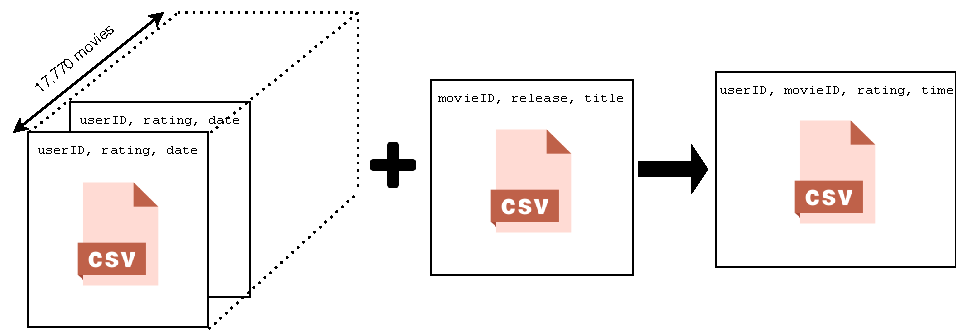
\includegraphics[width=\linewidth]{processing.pdf}
\end{figure}
%	\begin{block}{Title}
%		\begin{itemize}
%			\item test
%			\item item2
%		\end{itemize}
%	\end{block}
\end{frame}

\begin{frame}{Data filtering}
	\begin{enumerate}
		\item Discard MovieLens entries based on timestamps.
		\item Discard all movies not present on both datasets. A movie was uniquely identified by its title and release date.
		
		\faWarning "Lord of the Rings, The" and "The Lord of the Rings (2001)"
		
		\item Recast timestamps: from YYYY-MM-DD and elapsed seconds to common reference.
		\item Rounded MovieLens ratings.
	\end{enumerate}

	\vspace{0.5cm}
	\begin{centering}
	\hspace{.25\linewidth}\begin{minipage}{.5\linewidth}
		
		$\Longrightarrow$ 5800 common movies, 52,875 users remaining in ML and 478,756 in Netflix.
		
	
	\end{minipage}
\end{centering}
	
\end{frame}

